
% \begin{name}
% 	{\tenchude}
% 	{\tendethi}
% 	{\tentruong}
% 	{\thoigian}
% \end{name}
\Opensolutionfile{ans}[ans/ans-de21-7]

\begin{ex}%Câu 35.
Cho số phức $z$ thỏa mãn $3(\bar{z}+i)-(2-i) z=3+10 i$. Mô đun của z bằng
\choice
{$3$}
{$5$}
{\True $\sqrt{5}$}
{$\sqrt{3}$}

\end{ex}
\begin{ex}%Câu 1.
Trong không gian $O x y z$, cho điểm $I(2; 4;-3)$. Phương trình mặt cầu có tâm $I$ và tiếp xúc với mặt phẳng $(O x z)$ là
\choice
{$(x-2)^2+(y-4)^2+(z+3)^2=4$}
{$(x-2)^2+(y-4)^2+(z+3)^2=29$}
{$(x-2)^2+(y-4)^2+(z+3)^2=9$}
{\True $(x-2)^2+(y-4)^2+(z+3)^2=16$}

\end{ex}
\begin{ex}%Câu 2.
Trong không gian $O x y z$,cho mặt phẳng $(P)\colon x+2 y+3 z-1=0$. Vectơ nào dưới đây là một vectơ pháp tuyến của $(P)$ 
\choice
{$\vec{n}_3=(1; 2;-1)$}
{\True $\vec{n}_4=(1; 2; 3)$}
{$\vec{n}_1=(1; 3;-1)$}
{$\vec{n}_2=(2; 3;-1)$}

\end{ex}
\begin{ex}%Câu 3.
Với $a$ là số thực dương tùy ý, $\log_5 a^2$ bằng
\choice
{\True $2\log_5 a$}
{$2+\log_5 a$}
{$\dfrac{1}{2}+\log_5 a$}
{$\dfrac{1}{2} \log_5 a$}

\end{ex}
\begin{ex}%Câu 4.
\immini{
Cho hàm số $f(x)$ có bảng biến thiên như hình bên. Hàm số đã cho nghịch biến trên khoảng nào dưới đây?
}
{\vspace{-0.5cm}

\begin{tikzpicture}
\tkzTabInit[nocadre,lgt=1.2,espcl=1.4,deltacl=0.6]
{$x$/0.6,$f'(x)$/0.6,$f(x)$/1.8}{$-\infty$,$-2$,$0$,$2$,$+\infty$}
\tkzTabLine{,-,0,+,0,-,0,+,}
\tkzTabVar{+/$+\infty$,-/$1$,+/$3$,-/$1$,+/$+\infty$}
\end{tikzpicture}
}
\choice
{$(-2; 0)$}
{$(2;+\infty)$}
{\True $(0; 2)$}
{$(0;+\infty)$}
\end{ex}
\begin{ex}%Câu 5.
Nghiệm của phương trình $3^{2 x-1}=27$ là
\choice
{$x=5$}
{$x=1$}
{\True $x=2$}
{$x=4$}

\end{ex}
\begin{ex}%Câu 6.
Cho cấp số cộng $\left(u_n\right)$ với $u_1=3$ và $u_2=9$. Công sai của cấp số cộng đã cho bằng
\choice
{$-6$}
{$3$}
{$12$}
{\True $6$}

\end{ex}
\begin{ex}%Câu 7.
\immini{
Đồ thị của hàm số nào dưới đây có dạng như đường cong trong hình vẽ bên?
\choice
{\True $y=x^3-3 x^2+3$}
{$y=-x^3+3 x^2+3$}
{$y=x^4-2 x^2+3$}
{$y=-x^4+2 x^2+3$}}
{\vspace{-0.5cm}
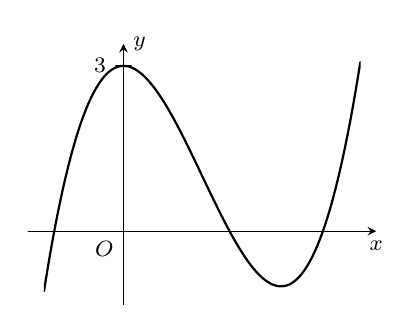
\begin{tikzpicture}[scale=1, font=\footnotesize, line join=round, line cap=round, >=stealth,y=0.7cm]
\def\xmin{-1.01}\def\xmax{3.01}\def\ymin{-1.13}\def\ymax{3.2}
\draw[->] (\xmin-0.2,0)--(\xmax+0.2,0) node[below] {\footnotesize $x$};
\draw[->] (0,\ymin-0.2)--(0,\ymax+0.2) node[right] {\footnotesize $y$};
\draw (0,0) node [below left] {\footnotesize $O$};
\foreach \x in {}\draw (\x,0.1)--(\x,-0.1) node [below] {\footnotesize $\x$};
\foreach \y in {3}\draw (0.1,\y)--(-0.1,\y) node [left] {\footnotesize $\y$};
\clip (\xmin,\ymin) rectangle (\xmax,\ymax);
\draw[thick,smooth,samples=200,domain=\xmin:\xmax] plot (\x,{1*((\x)^3)+-3*((\x)^2)+0*(\x)+3});
\end{tikzpicture}
}

\end{ex}
\begin{ex}%Câu 8.
Trong không gian $O x y z$, cho đường thẳng $d\colon \dfrac{x-2}{-1}=\dfrac{y-1}{2}=$ $\dfrac{z+3}{1}$. Vectơ nào dưới đây là một vectơ chỉ phương của $d$?
\choice
{$\overrightarrow{u_2}=(2; 1; 1)$}
{$\overrightarrow{u_4}=(1; 2;-3)$}
{\True $\overrightarrow{u_3}=(-1; 2; 1)$}
{$\overrightarrow{u_1}=(2; 1;-3)$}

\end{ex}
\begin{ex}%Câu 9.
Thể tích của khối nón có chiều cao $h$ và bán kính $r$ là
\choice
{\True $\dfrac{1}{3} \pi r^2 h$}
{$\pi r^2 h$}
{$\dfrac{4}{3} \pi r^2 h$}
{$2\pi r^2 h$}

\end{ex}
\begin{ex}%Câu 10.
Số cách chọn $2$ học sinh từ $7$ học sinh là
\choice
{$2^7$}
{$A_7^2$}
{\True $C_7^2$}
{$7^2$}

\end{ex}
\begin{ex}%Câu 11.
Trong không gian $O x y z$, hình chiếu vuông góc của điểm $M(2; 1;-1)$ trên trục $O z$ có tọa độ là
\choice
{$(2; 1; 0)$}
{\True $(0; 0;-1)$}
{$(2; 0; 0)$}
{$(0; 1; 0)$}

\end{ex}
\begin{ex}%Câu 12.
Biết $\displaystyle\int\limits_0^1 f(x) \mathrm{d} x=-2$ và $\displaystyle\int\limits_0^1 g(x) \mathrm{d} x=3$, khi đó $\displaystyle\int\limits_0^1[f(x)-g(x)] \mathrm{d} x$ bằng
\choice
{\True $-5$}
{$5$}
{$-1$}
{$1$}

\end{ex}
\begin{ex}%Câu 13.
Thể tích khối lăng trụ có diện tích đáy $B$ và chiều cao $h$ là
\choice
{$3 B h$}
{\True $Bh$}
{$\dfrac{4}{3} B h$}
{$\dfrac{1}{3} B h$}

\end{ex}
\begin{ex}%Câu 14.
Số phức liên hợp của số phức $3-4 i$ là.
\choice
{$-3-4 i$}
{$-3+4 i$}
{\True $3+4 i$}
{$-4+3 i$}

\end{ex}
\begin{ex}%Câu 15.
\immini{
Cho hàm số $f(x)$ có bảng biến thiên như hình bên. Hàm số đã cho đạt cực tiểu tại.
\choice
{$x=2$}
{$x=1$}
{\True $x=-1$}
{$x=-3$}}
{

\begin{tikzpicture}
\tkzTabInit[nocadre,lgt=1.2,espcl=1.6,deltacl=0.6]
{$x$/0.6,$f'(x)$/0.6,$f(x)$/1.8}{$-\infty$,$-1$,$2$,$+\infty$}
\tkzTabLine{,-,0,+,0,-,}
\tkzTabVar{+/$+\infty$,-/$-3$,+/$1$,-/$-\infty$}
\end{tikzpicture}

}

\end{ex}
\begin{ex}%Câu 16.
Họ tất cả các nguyên hàm của hàm số $f(x)=2 x+5$ là:
\choice
{\True $x^2+5 x+C$}
{$2 x^2+5 x+C$}
{$2 x^2+C$}
{$x^2+C$}

\end{ex}
\begin{ex}%Câu 17.
\immini{
Cho hàm số $y=f(x)$ có bảng biến thiên như hình bên. Số nghiệm thực của phương trình $2 f(x)-3=0$ là:
}
{\vspace{-0.5cm}

\begin{tikzpicture}
\tkzTabInit[nocadre,lgt=1.2,espcl=1.4,deltacl=0.6]
{$x$/0.6,$f'(x)$/0.6,$f(x)$/1.8}{$-\infty$,$-2$,$0$,$2$,$+\infty$}
\tkzTabLine{,+,0,-,0,+,0,-,}
\tkzTabVar{-/$-\infty$,+/$3$,-/$-1$,+/$3$,-/$-\infty$}
\end{tikzpicture}
}
\choice
{$2$}
{$1$}
{\True $4$}
{$3$}
\end{ex}
\begin{ex}%Câu 18.
Cho hình chóp $S.ABC$ có $SA$ vuông góc với mặt phẳng\\ $(ABC), SA=$ $2 a$, tam giác $ABC$ vuông tại $B, AB=a \sqrt{3}$ và $BC=a$. Góc giữa đường thẳng $SC$ và mặt phẳng $(ABC)$ bằng
\choice
{$90^{\circ}$}
{\True $45^{\circ}$}
{$30^{\circ}$}
{$60^{\circ}$}

\end{ex}
\begin{ex}%Câu 19.
Gọi $z_1, z_2$ là hai nghiệm phức của phương trình $z^2-6 z+10=0$. Giá trị của $z_1^2+z_2^2$ bằng
\choice
{\True $16$}
{$56$}
{$20$}
{$26$}

\end{ex}
\begin{ex}%Câu 20.
Hàm số $y=2^{x^2-3 x}$ có đạo hàm là
\choice
{\True $(2 x-3) 2^{x^2-3 x} \cdot \ln 2$}
{$2^{x^2-3 x} \cdot \ln 2$}
{$(2 x-3) 2^{x^2-3 x}$}
{$(2 x-3) 2^{x^2-3 x-1}$}

\end{ex}
\begin{ex}%Câu 21.
Giá trị lớn nhất của hàm số $f(x)=x^3-3 x+2$ trên đoạn $[-3; 3]$ bằng
\choice
{$-16$}
{\True $20$}
{$0$}
{$4$}

\end{ex}
\begin{ex}%Câu 22.
Trong không gian $O x y z$, cho mặt cầu $(S)\colon x^2+y^2+z^2+2 x-$ $2 z-7=0$. Bán kính của mặt cầu đã cho bằng
\choice
{$\sqrt{7}$}
{$9$}
{\True $3$}
{$\sqrt{15}$}

\end{ex}
\begin{ex}%Câu 23.
Cho khối chóp đứng $ABC \cdot A'B'C'$ có đáy là tam giác đều cạnh $a$ và $AA'=a \sqrt{3}$. Thể tích của khối lăng trụ đã cho bằng
\choice
{\True $\dfrac{3 a^3}{4}$}
{$\dfrac{3 a^3}{2}$}
{$\dfrac{a^3}{4}$}
{$\dfrac{a^3}{2}$}

\end{ex}
\begin{ex}%Câu 24.
Cho hàm số $y=f(x)$ có đạo hàm $f'(x)=x(x+2)^2, \forall x \in \mathbb{R}$. Số điểm cực trị của hàm số đã cho là.
\choice
{$0$}
{$3$}
{$2$}
{\True $1$}

\end{ex}
\begin{ex}%Câu 25.
Cho $a, b$ là hai số thực dương thỏa mãn $a^4 b=16$. Giá trị $4\log_2 a+$ $\log_2 b$ bằng
\choice
{\True $4$}
{$2$}
{$16$}
{$8$}

\end{ex}
\begin{ex}%Câu 26.
Cho hai số phức $z_1=1-i$ và $z_2=1+2 i$. Trên mặt phẳng $O x y$, điểm biểu diễn số phức $3 z_1+z_2$ có tọa độ là
\choice
{\True $(4;-1)$}
{$(-1; 4)$}
{$(4; 1)$}
{$(1; 4)$}

\end{ex}
\begin{ex}%Câu 27.
Nghiệm của phương trình $\log_3(x+1)+1=\log_3(4 x+1)$ là
\choice
{$x=3$}
{$x=-3$}
{$x=4$}
{\True $x=2$}

\end{ex}

\begin{ex}%Câu 28.
Mặt cầu ngoại tiếp hình lập phương cạnh $a$ thì có diện tích bằng:
\choice
{$a^3$}
{$\dfrac{4\pi a^3}{3}$}
{\True $3\pi a^2$}
{$12\pi a^2 \sqrt{3}$}

\end{ex}
\begin{ex}%Câu 29.
\immini{
Cho hàm số $y= f(x)$ có bảng biến thiên như hình bên. Tổng số đường tiệm cận đứng và tiệm cận ngang của đồ thị hàm số đã cho là
}
{
	
\begin{tikzpicture}[scale=1,line width=.6pt]
\tkzTabInit[nocadre=true,lgt=1,espcl=1.6,deltacl=0.5,lw=0.8]
{$x$ /.7,$f'(x)$/.7,$f(x)$/1.8}{$-\infty$,$0$,$1$,$+\infty$}
\tkzTabLine{,-,d,-,0,+,}
\tkzTabVar{+/$2$,-D+/$-4$/$+\infty$,-/$-2$,+/$+\infty$}
\end{tikzpicture}
}
\choice
{$4$}
{$1$}
{$3$}
{\True $2$}
\end{ex}
\begin{ex}%Câu 30.
\immini{
Gọi $S$ là diện tích hình phẳng giới hạn bởi đồ thị hàm số $y=f(x)$, trục hoành, $x=a, x=b$. Khi đó $S$ được tính theo công thức nào dưới đây?}
{\begin{tikzpicture}[>=stealth, scale=1,samples=200,smooth,line width=.6pt,xscale=1,yscale=1]
\tikzstyle{every node}=[font=\small]
\pgfmathsetmacro{\a}{sqrt(2)}
 \draw[->,thick] (-0.5,0)--(6,0) node[above] {$x$};
 \draw[->,thick] (0,-1)--(0,1) node[right] {$y$};
 \draw (0,0) node [above right] {$O$};
 \foreach \x in {}
\draw[thin] (\x,1pt)--(\x,-1pt) node [below] {$\x$};
 \foreach \y in {}
 	\draw[thin] (1pt,\y)--(-1pt,\y) node [left] {$\y$};
 \begin{scope}
\draw[domain=0.62:5.38,smooth,variable=\x]
plot (\x,{-1/4*(\x)^3+9/4*(\x)^2-23/4*(\x)+15/4})node[right]{$y=f(x)$};
 \fill[pattern=north east lines,smooth,pattern color=blue] (1,0)--plot[domain=1:5] (\x,{-1/4*(\x)^3+9/4*(\x)^2-23/4*(\x)+15/4})--(5,0)--cycle;
\end{scope}
\path
(1,0)  node[above, xshift=0.1cm]{$a$}
(3,0)  node[above, xshift=0cm]{$c$}
(5,0)  node[below, xshift=-0.1cm]{$c$}
;
\end{tikzpicture}
}
\choice
{$S=\displaystyle\int\limits_a^{b} f(x) \mathrm{d} x$}
{$S=\displaystyle\int\limits_a^{c} f(x) \mathrm{d} x+\displaystyle\int\limits_c^{b} f(x) \mathrm{d} x$}
{\True $S=-\displaystyle\int\limits_a^{c} f(x) \mathrm{d} x+\displaystyle\int\limits_c^{b} f(x) \mathrm{d} x$}
{$S=\left|\displaystyle\int\limits_a^{c} f(x) \mathrm{d} x+\displaystyle\int\limits_c^{b} f(x) \mathrm{d} x\right|$}

\end{ex}
\begin{ex}%Câu 31.
Trong không gian $O x y z$, cho hai điểm $A(1; 3; 0)$ và $B(5; 1;-2)$.
Mặt phẳng trung trực của đoạn thẳng $AB$ có phương trình là
\choice
{$2 x-y-z+5=0$}
{\True $2 x-y-z-5=0$}
{$x+2 y+2 z-3=0$}
{$3 x+2 y-z-14=0$}

\end{ex}
\begin{ex}%Câu 32.
Họ tất cả các nguyên hàm của hàm số $f(x)=\dfrac{2 x-1}{(x+1)^2}$ trên khoảng $(-1;+\infty)$ là
\choice
{$2\ln (x+1)+\dfrac{2}{x+1}+C$}
{\True $2\ln (x+1)+\dfrac{3}{x+1}+C$}
{$2\ln (x+1)-\dfrac{2}{x+1}+C$}
{$2\ln (x+1)-\dfrac{3}{x+1}+C$}

\end{ex}
\begin{ex}%Câu 33.
Cho hàm số $f(x)$. Biết $f(0)=4$ và $f'(x)=2\cos ^2 x+1, \forall x \in \mathbb{R}$,
khi đó $\displaystyle\int\limits_0^{\frac{\pi}{4}} f(x)\mathrm{\,d}x$ bằng
\choice
{$\dfrac{\pi^2+4}{16}$}
{$\dfrac{\pi^2+14\pi}{16}$}
{\True $\dfrac{\pi^2+16\pi+4}{16}$}
{$\dfrac{\pi^2+16\pi+16}{16}$}

\end{ex}
\begin{ex}%Câu 34.
Trong không gian $O x y z$, cho các điểm $A(1; 2; 0), B(2; 0; 2)$\\
,$C(2;-1; 3), D(1; 1; 3)$. Đường thẳng đi qua $C$ và vuông góc với mặt phẳng $(ABD)$ có phương trình là
\choice
{$\heva{&x=4+2 t \\& y=3-t \\& z=1+3 t}$}
{$\heva{&x=4+2 t \\& y=3-t \\& z=1+3 t}$}
{\True $\heva{&x=4+2 t \\& y=3-t \\& z=1+3 t}$}
{$\heva{&x=4+2 t \\& y=3-t \\& z=1+3 t}$}

\end{ex}

\begin{ex}%Câu 36
Cho hàm số $f(x)$, bảng xét dâu của $f'(x)$ như sau:
\immini{
Hàm số $y=f(3-2 x)$ nghịch biến trên khoảng nào dưới đây?
}
{

\begin{tikzpicture}[scale=1,line width=.6pt]
\tkzTabInit[nocadre=true,lgt=1,espcl=1.4,deltacl=0.5,lw=0.8]
{$x$ /.7,$y'$/.7}{$-\infty$,$-3$,$-1$,$1$,$+\infty$}
\tkzTabLine{,-,0,+,0,-,0,+,}
\end{tikzpicture}
}
\choice
{$(4;+\infty)$}
{\True $(-2; 1)$}
{$(2; 4)$}
{$(1; 2)$}
\end{ex}
\begin{ex}%Câu 37.
\immini{
Cho hàm số $f(x)$ có bảng biến thiên như hình bên.
Số nghiệm thực của phương trình $2 f(x)-\sqrt{10}=0$ là
}
{

\begin{tikzpicture}
\tkzTabInit[nocadre,lgt=1.2,espcl=1.4,deltacl=0.6]
{$x$/0.6,$f'(x)$/0.6,$f(x)$/1.8}{$-\infty$,$-2$,$0$,$2$,$+\infty$}
\tkzTabLine{,-,0,+,0,-,0,+,}
\tkzTabVar{+/$+\infty$,-/$-1$,+/$2$,-/$-1$,+/$-\infty$}
\end{tikzpicture}
}
\choice
{$3$}
{$2$}
{$0$}
{\True $4$}
\end{ex}
\begin{ex}%Câu 38.
Cho khối hộp chữ nhật $ABCD \cdot A'B'C'D'$ có các cạnh $AB=a, AD=a \sqrt{2}, AA'=a \sqrt{5}$. Thể tích của khối hộp đó là
\choice
{$\dfrac{a^3 \sqrt{10}}{2}$}
{\True $a^3 \sqrt{10}$}
{$a^2 \sqrt{10}$}
{$\dfrac{a^3 \sqrt{10}}{3}$}
\end{ex}
\begin{ex}%Câu 39.
Cho cấp số nhân $\left(u_n\right)$ với $u_1=2$ và $u_2=8$. Công bội của cấp số nhân đã cho bằng
\choice
{$10$}
{$-6$}
{\True $4$}
{$6$}
\end{ex}
\begin{ex}%Câu 40.
Cho hình nón có đường sinh bằng $4 a$, diện tích xung quanh bằng $8\pi a^2$. Tính chiều của hình nón đó theo $a$.
\choice
{$2 a$}
{$a \sqrt{3}$}
{\True $2 a \sqrt{3}$}
{$\dfrac{a \sqrt{3}}{3}$}
\end{ex}
\begin{ex}%Câu 41.
Tập xác định của hàm số $y=\left(3^{x}-9\right)^{-2}$ là
\choice
{\True $D=\mathbb{R} \backslash\{2\}$}
{$D=\mathbb{R} \backslash\{0\}$}
{$(2;+\infty)$}
{$(0;+\infty)$}
\end{ex}
\begin{ex}%Câu 42.
Một hình trụ có bán kính đáy bằng $50\mathrm{\,cm}$ và chiều cao bằng $50\mathrm{\,cm}$. Diện tích xung quanh của hình trụ bằng:
\choice
{$7500\pi\left(\mathrm{cm}^2\right)$}
{$2500\pi\left(\mathrm{cm}^2\right)$}
{\True $5000\pi\left(\mathrm{cm}^2\right)$}
{$10000\pi\left(\mathrm{cm}^2\right)$}
\end{ex}
\begin{ex}%Câu 43.
Đồ thị hàm số nào sau đây không có tiệm cận đứng?
\choice
{$y=\dfrac{\sqrt{x+3}}{x+2}$}
{\True $y=\dfrac{3 x-1}{x^2+1}$}
{$y=\dfrac{1}{x^2-2 x+1}$}
{$y=\dfrac{-1}{x^2}$}

\end{ex}
\begin{ex}%Câu 44.
Họ nguyên hàm của hàm số $f(x)={\rm e}^{x}\left(3+{\rm e}^{-x}\right)$.
\choice
{$F(x)=3 {\rm e}^{x}-x+C$}
{\True $F(x)=3 {\rm e}^{x}+x+C$}
{$F(x)=3 {\rm e}^{x}+{\rm e}^{x} \ln {\rm e}^{x}+C$}
{$F(x)=3 {\rm e}^{x}-\dfrac{1}{{\rm e}^{x}}+C$}

\end{ex}
\begin{ex}%Câu 45.
Với $a$ là số nguyên dương tùy ý, $\log_{\frac{1}{2}} a^3$ bằng
\choice
{$3-\log_2 a$}
{$\dfrac{3}{2} \log_2 a$}
{\True $-3\log_2 a$}
{$3\log_2 a$}

\end{ex}
\begin{ex}%Câu 46.
\immini{
Cho hàm số $y=f(x)$ có bảng biến thiên như hình bên dưới.
Hàm số đã cho đạt cực tiểu tại
\choice
{$x=2$}
{$x=-2$}
{$x=3$}
{\True $x=1$}}
{\vspace{-0.5cm}

\begin{tikzpicture}
\tkzTabInit[nocadre,lgt=1.2,espcl=1.6,deltacl=0.6]
{$x$/0.6,$f'(x)$/0.6,$f(x)$/1.8}{$-\infty$,$1$,$3$,$+\infty$}
\tkzTabLine{,-,0,+,0,-,}
\tkzTabVar{+/$+\infty$,-/$-2$,+/$2$,-/$-\infty$}
\end{tikzpicture}

}

\end{ex}
\begin{ex}%Câu 47.
Nghiệm của phương trình $5^{2 x+1}=125$ là
\choice
{$x=2$}
{\True $x=1$}
{$x=5$}
{$x=4$}

\end{ex}
\begin{ex}%Câu 48.
\immini{
Đồ thị của hàm số nào dưới đây có dạng như đường cong trong hình bên?
\choice
{$y=x^3+4 x^2-1$}
{$y=-x^4+4 x^2+1$}
{\True $y=-\dfrac{1}{3} x^3+2 x+1$}
{$y=\dfrac{1}{3} x^3-2 x+1$}}
{\vspace{0.5cm}
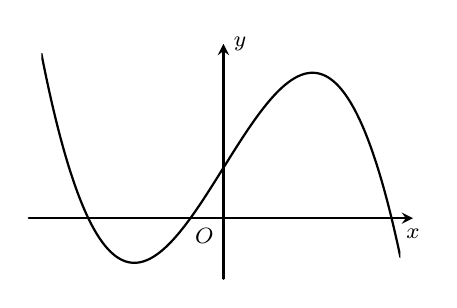
\begin{tikzpicture}[scale=.8, font=\footnotesize, line join=round, line cap=round, >=stealth,y=0.8cm]
\def\xmin{-2.89}\def\xmax{2.81}\def\ymin{-1}\def\ymax{3.26}
\draw[->,thick] (\xmin-0.2,0)--(\xmax+0.2,0) node[below] {\footnotesize $x$};
\draw[->,thick] (0,\ymin-0.2)--(0,\ymax+0.2) node[right] {\footnotesize $y$};
\draw (0,0) node [below left] {\footnotesize $O$};
\foreach \x in {}\draw (\x,0.1)--(\x,-0.1) node [below] {\footnotesize $\x$};
\foreach \y in {}\draw (0.1,\y)--(-0.1,\y) node [left] {\footnotesize $\y$};
\clip (\xmin,\ymin) rectangle (\xmax,\ymax);
\draw[thick,smooth,samples=200,domain=\xmin:\xmax] plot (\x,{-1/3*((\x)^3)+0*((\x)^2)+2*(\x)+1});
\end{tikzpicture}
}

\end{ex}
\begin{ex}%Câu 49.
Một tổ có $6$ học sinh nam và $9$ học sinh nữ. Hỏi có bao nhiêu cách chọn $1$ học sinh nam và 1 học sinh nữ đi lao động?
\choice
{$C_6^1+C_{15}^1$}
{\True $C_6^1 C_9^1$}
{$C_6^1+C_9^1$}
{$C_6^1 C_{15}^1$}

\end{ex}

\begin{ex}%Câu 50.
Mặt cầu ngoại tiếp hình lập phương cạnh $a$ thì có diện tích bằng:
\choice
{$a^3$}
{$\dfrac{4\pi a^3}{3}$}
{\True $3\pi a^2$}
{$12\pi a^2 \sqrt{3}$}

\end{ex}

\Closesolutionfile{ans}
%% \indapan{10}{ans/ans-de21-7}